---
title: Part 13 Dependency inversion
author: Dimitri Merejkowsky
date: EFREI 2022-2023
---


# Dependency inversion

## Setup

* A PostgreSQL database containing employee records.
* A Web application that needs to display information about an employee
  given its ID number.

## Classes diagram

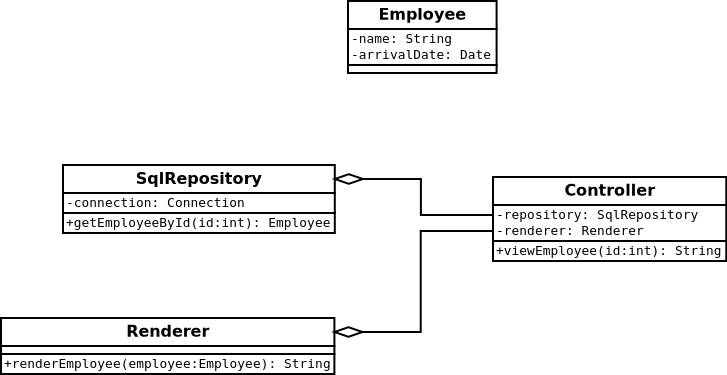
\includegraphics[width=10cm]{img/uml/employee-render-1.png}

## Code


```java
import SQLRepository;
import Renderer;

public class Controller {
    private SQLRepository repository;
    private Renderer renderer;

    public Controller() {
        repository = new SQLRepository();
        renderer = new Renderer();
    }

    public String viewEmployee(int id) {
        Employee employee = repository.getEmployeeByID(id);
        String res = renderer.renderEmployee(employee);
        return res;
    }
}
```

## Testing the Controller

* We need a real sql connection to build an Controller
* There's a temporal dependency between the SQL connection and the Controller
* There's *also* a *source* dependency between the two

\vfill

It's hard to test!

## Solution - UML


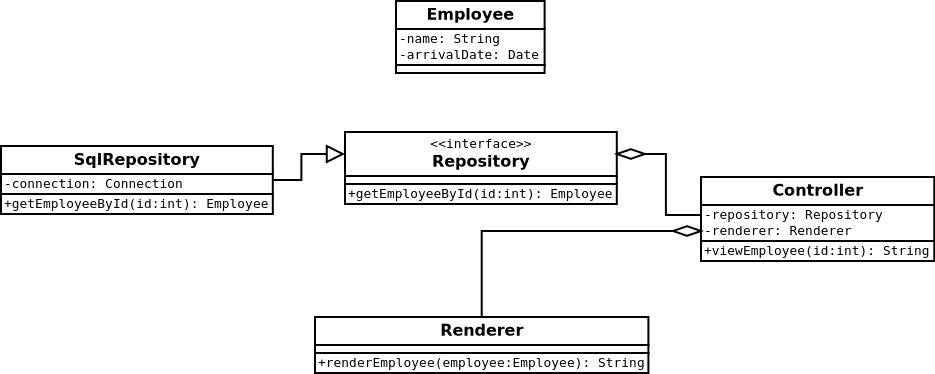
\includegraphics[width=10cm]{img/uml/employee-render-2.png}

## Solution - in code

```java
// In Repository.java
public interface Repository {
    public Employee getEmployeeByID(int id);
}
```

```diff
// In SQLRepository.java
+import Repository;

-public class SQLRepository {
+public class SQLRepository implements Repository {
}
```

## Solution - in code

```diff
-import SQLRepository;
+import Repository;
 import Renderer;

 public class Controller {
-    private SQLRepository repository;
+    private Repository repository;
     private Renderer renderer;

-    public Controller() {
-        this.repository = new SQLRepository();
-        this.renderer = new Renderer();
-   }

+    public Controller(Repository repository) {
+        this.repository = repository;
+        this.renderer = new Renderer();
+    }
```

## Dependency Inversion

There is still a *temporal* dependency between `Controller` and `SQLRepository`

But now there's a *source dependency* from `SQLRepository` to `Repository`
*in the other direction*.

This is called `dependency inversion` (or DI) and it's a very cool technique


## Adding a FakeRepository

```java
public class FakeRepository implements Repository {
    private ArrayList<Employee> employees;

    public FakeRepository() {
        employees = new ArrayList<Employee>();
    }

    public void addEmployee(Employee employee) {
        employees.add(employee);
    }

    public Employee getEmployeeByID(int id) {
        return employees.get(id);
    }
}
```

## As UML


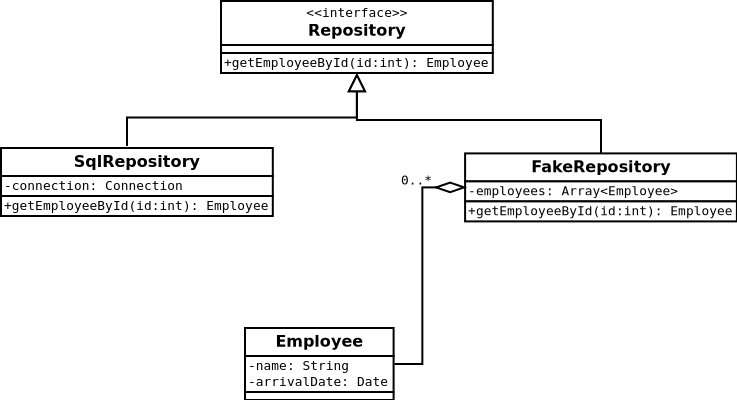
\includegraphics[width=10cm]{img/uml/employee-render-3.png}

## Testing with the FakeRepository

\small

```java
public class ControllerTest {
    @Test
    public void testViewEmployee() {
        Employee smith = new Employee("John Smith");

        FakeRepository fakeRepository = new FakeRepository();
        fakeRepository.addEmployee(smith);

        Controller controller = new Controller(fakeRepository);

        String html = controller.viewEmployee(0);
        assertEquals(html,
            "<span class=\"employee\">John Smith</span>"
        );
    }
}
```

## Question for you

Should we introduce an interface for the Renderer class too?

## main

The only place that needs *all* the sources and temporal dependencies


```java
import Repository, SQLRepository;
import Controller;

public static void main(String[] args) {
    Connection connection = ...;
    Repository repository = SQLRepository(connection);

    Controller controller = new Controller(repository);
}
```

## Boundaries

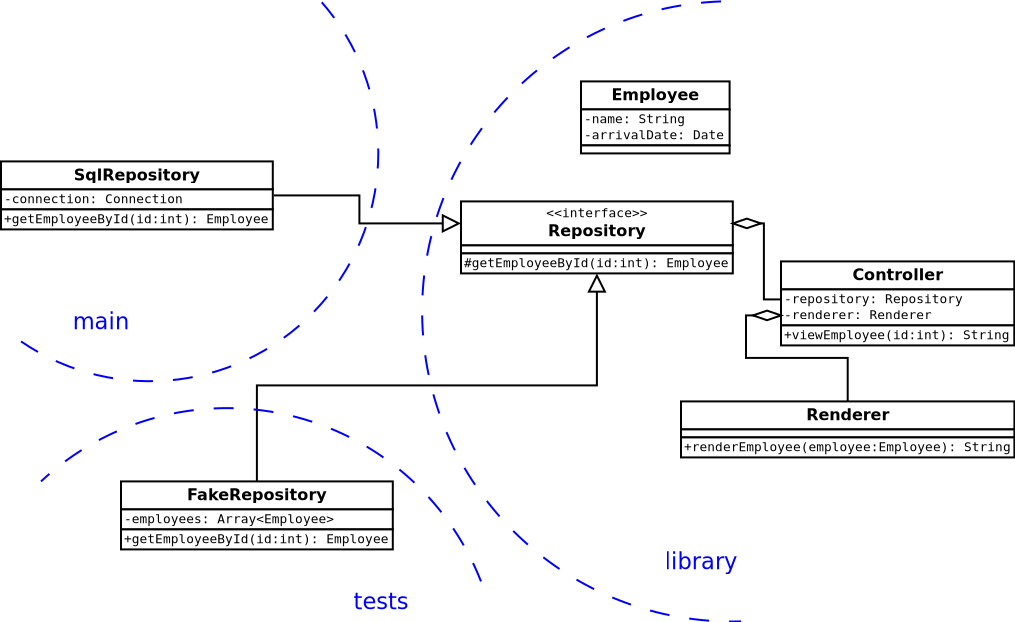
\includegraphics[width=10cm]{img/uml/boundaries.png}

# Interfaces

## Explicit interfaces

In Java, C# and Typescript

## Implicit interfaces

You can do it like this:

```python
class FakeRepository:

    def add_employee(self, employee):
        ...

    def get_employee_by_id(self, id):
        ...
```

The class *happen* to have a common same set of methods.

Python calls this a *protocol*


## Duck typing

![](img/duck-cow.jpg)

## Using a base class - old way

```python
class Repository():
    def get_employee_by_id(self, id):
        raise NotImplementedError()

class FakeRepository(Repository):
    def get_employee_by_id(self, id)
```

\vfill

You'll get a runtime error when `get_employee_by_id()` is called.


## Using a base class - new way

```python
import abc
class Repository(metaclass=abc.ABCMeta):
    @abc.abstracmethod
    def get_employee_by_id(self, id):
        raise NotImplementedError()

class FakeRepository(Repository):
    def get_employee_by_id(self, id)
```

\vfill

You'll get an error when `FakeRepository()` is instantiated,
which is sooner than with the old way.

Coders coming from other languages won't be surprised.

## The hype way

Use type annotations and a type checker, like
`flow` or `typescript` (for javascript) - or
`mypy` (for Python)
